\chapter{Enóis, enolatos e a reação aldólica}\label{ch:b2:enolates-aldol}

Cada vez que uma célula degrada a glicose, uma enzima corta um fosfato de
açúcar de seis carbonos em dois pedaços de três carbonos: uma reação \omterm{def:b2:enolates-aldol:aldol}{aldólica}
conduzida ao contrário. No sentido direto, a mesma reação junta dois compostos
carbonílicos em um só, e é o meio mais usado pelos químicos para criar
ligações carbono--carbono. Ela repousa sobre uma propriedade que os capítulos
anteriores apenas tocaram: os átomos de hidrogênio vizinhos de um grupo
carbonila são ácidos, e retirar um deles transforma o carbono ao lado da
carbonila em nucleófilo.

\begin{recall}
O volume do 1.º ano: $\mathrm pK_a$ e a reação prevalente, carbânions, controle cinético e
termodinâmico, \omterm{def:b2:amines:nucleophilic-addition}{adições nucleofílicas} às carbonilas, eliminações E1 e E2, a hidratação dos
alcinos (um \omterm{def:b2:enolates-aldol:tautomerism}{enol} que se rearranja). \Cref{ch:b2:frontier-orbitals}: \omterm{def:b2:frontier-orbitals:ambident}{nucleófilos ambidentados}.
\Cref{ch:b2:acyl-substitution}: ésteres e substituição acílica.
\end{recall}

\section{A tautomeria ceto--enólica}

\begin{definition}[Tautomeria]\label{def:b2:enolates-aldol:tautomerism}
\emph{Tautômeros}\index{tautomeros@tautômeros} são isômeros que se interconvertem pelo deslocamento de um
hidrogênio e de uma ligação dupla. Na \emph{tautomeria ceto--enólica}\index{tautomeria ceto--enolica@tautomeria ceto--enólica}, um composto
carbonílico com um hidrogênio no carbono vizinho da carbonila (a forma ceto) está em equilíbrio com
seu \emph{enol}\index{enol}, um álcool levado por uma ligação dupla \ce{C=C}.
\end{definition}

\begin{omfigure}
\setchemfig{atom sep=2em}
\schemestart
\chemfig{H_3C-C(=[2]O)-CH_3}
\arrow{<=>[\ce{H+} ou \ce{HO-}][catálise]}[,2.2]
\chemfig{H_3C-C(-[2]OH)=CH_2}
\schemestop
\par\vspace{6pt}

{\small A propanona e seu \omterm{def:b2:enolates-aldol:tautomerism}{enol}, o prop-1-en-2-ol. O ácido (protonação do oxigênio carbonílico, depois
perda de um hidrogênio $\alpha$) ou a base (remoção de um hidrogênio $\alpha$, depois protonação do
oxigênio) catalisa a interconversão; o equilíbrio fica muito do lado da forma ceto.}
\end{omfigure}

\begin{proposition}[Teor de enol]\label{prop:b2:enolates-aldol:enol-content}
Os aldeídos e cetonas simples contêm apenas traços de \omterm{def:b2:enolates-aldol:tautomerism}{enol}; os compostos 1,3-dicarbonílicos, como a
pentano-2,4-diona, contêm uma grande proporção dele.
\end{proposition}

\begin{proof}[Raciocínio]
Uma ligação \ce{C=O} é mais forte que uma ligação \ce{C=C} por mais do que uma ligação \ce{O-H} é mais
fraca que uma ligação \ce{C-H}: a forma ceto é favorecida. Em um composto 1,3-dicarbonílico, a ligação
dupla do \omterm{def:b2:enolates-aldol:tautomerism}{enol} é conjugada com o segundo grupo carbonila, e o \ce{OH} do \omterm{def:b2:enolates-aldol:tautomerism}{enol} forma uma ligação de
hidrogênio interna com seu oxigênio, em um anel de seis membros: ambos estabilizam o \omterm{def:b2:enolates-aldol:tautomerism}{enol} o bastante
para fazer dele uma forma majoritária.
\end{proof}

Como o \omterm{def:b2:enolates-aldol:tautomerism}{enol} é plano em sua \ce{C=C}, um estereocentro no carbono $\alpha$ se perde cada vez que o
\omterm{def:b2:enolates-aldol:tautomerism}{enol} se forma: uma cetona opticamente ativa com um estereocentro vizinho de sua carbonila racemiza em
meio ácido ou básico.

\section{Os enolatos}

\begin{definition}[Enolatos]\label{def:b2:enolates-aldol:enolate}
O \emph{carbono $\alpha$}\index{carbono alfa@carbono $\alpha$} de um composto carbonílico é o carbono
ligado ao carbono carbonílico; seus hidrogênios são os \emph{hidrogênios $\alpha$}\index{hidrogenio alfa@hidrogênio $\alpha$}.
Retirar um deles dá um \emph{íon enolato}\index{ion enolato@íon enolato}, cuja
carga negativa é compartilhada entre o carbono $\alpha$ e o oxigênio.
\end{definition}

\begin{proposition}[Acidez dos hidrogênios $\alpha$]\label{prop:b2:enolates-aldol:alpha-acidity}
Os hidrogênios $\alpha$ são muito mais ácidos que as ligações \ce{C-H} comuns, porque o \omterm{def:b2:enolates-aldol:enolate}{enolato} é
estabilizado por ressonância; um hidrogênio situado entre dois grupos carbonila é ácido o bastante
para ser retirado por um alcóxido ou até pelo hidróxido.
\end{proposition}

\begin{proof}[Raciocínio]
No \omterm{def:b2:enolates-aldol:enolate}{enolato}, a carga negativa fica em parte no oxigênio eletronegativo; uma segunda carbonila do
outro lado a deslocaliza sobre dois oxigênios. Medida em água, a pentano-2,4-diona tem $\mathrm pK_a =
9.0$ e o 3-oxobutanoato de etila 10.7, comparáveis ao nitrometano (10.2), cujo ânion é estabilizado
da mesma maneira pelo grupo nitro; uma cetona simples, com uma só carbonila, é muito mais fraca ---
fraca demais para que sua acidez seja medida diretamente em água.
% ledger: pka:acac, pka:acetoacetate, pka:nitromethane
\end{proof}

\begin{omfigure}
\setchemfig{atom sep=2em}
\schemestart
\chemfig{H_3C-C(=[2]O)-\chemabove{C}{\scriptstyle -}H_2}
\arrow{<->}
\chemfig{H_3C-C(-[2]\chemabove{O}{\scriptstyle -})=CH_2}
\schemestop
\par\vspace{6pt}

{\small As duas estruturas de ressonância do \omterm{def:b2:enolates-aldol:enolate}{enolato} da propanona. A carga negativa é compartilhada
pelo carbono $\alpha$ e pelo oxigênio: o \omterm{def:b2:enolates-aldol:enolate}{enolato} é um \omterm{def:b2:frontier-orbitals:ambident}{nucleófilo ambidentado}, que reage com a maioria
dos eletrófilos carbonados pelo carbono.}
\end{omfigure}

\begin{definition}[Enolatos cinético e termodinâmico]\label{def:b2:enolates-aldol:kinetic-enolate}
Para uma cetona com dois carbonos $\alpha$ diferentes, o \emph{enolato cinético}\index{enolato cinetico@enolato cinético}
é o que se forma mais depressa, por remoção de um hidrogênio do lado menos impedido e menos
substituído; o \emph{enolato termodinâmico}\index{enolato termodinamico@enolato termodinâmico} é o mais estável, com a ligação
dupla mais substituída.
\end{definition}

\begin{proposition}[Escolher o enolato]\label{prop:b2:enolates-aldol:enolate-control}
Uma base forte e volumosa, usada em quantidade total a baixa temperatura (di-isopropilamideto de
lítio, LDA, a \qty{-78}{\degreeCelsius}), forma o \omterm{def:b2:enolates-aldol:kinetic-enolate}{enolato cinético} de modo completo e irreversível; uma
base mais fraca à temperatura ambiente (um alcóxido em seu álcool) deixa os \omterm{def:b2:enolates-aldol:enolate}{enolatos} se
interconverterem e dá sobretudo o termodinâmico.
\end{proposition}

\begin{proof}[Raciocínio]
O LDA ($\mathrm pK_a$ da di-isopropilamina perto de 36, muito acima do da cetona) desprotona de
modo completo e rápido; a baixa temperatura, o \omterm{def:b2:enolates-aldol:enolate}{enolato} não é reprotonado, e a desprotonação mais
rápida, no \ce{CH2} ou no \ce{CH3} acessível, decide: controle cinético. Um alcóxido só retira o próton
em parte, os \omterm{def:b2:enolates-aldol:enolate}{enolatos} e a cetona trocam prótons continuamente, e a mistura de equilíbrio favorece o
\omterm{def:b2:enolates-aldol:enolate}{enolato} mais substituído, mais estável: controle termodinâmico (como no volume do 1.º ano).
% ledger: ghs:LDA
\end{proof}

\section{Alquilar os enolatos}

Os \omterm{def:b2:enolates-aldol:enolate}{enolatos} atacam os haloalcanos primários por substituição bimolecular, formando uma nova ligação
\ce{C-C} no carbono $\alpha$. Com os hidrogênios $\alpha$ muito ácidos de um composto 1,3-dicarbonílico,
um alcóxido basta, e a carbonila suplementar pode ser removida depois.

\begin{definition}[Descarboxilação]\label{def:b2:enolates-aldol:decarboxylation}
Uma \emph{descarboxilação}\index{descarboxilacao@descarboxilação} remove um grupo carboxila na forma de \ce{CO2}. Na
\emph{síntese malônica}\index{sintese malonica@síntese malônica}, o propanodioato de dietila é desprotonado,
alquilado, hidrolisado ao ácido propanodioico substituído e descarboxilado por aquecimento, dando
um ácido carboxílico \ce{RCH2COOH}.
\end{definition}

\begin{proposition}[Descarboxilações fáceis]\label{prop:b2:enolates-aldol:decarboxylation}
Os $\beta$-cetoácidos e os ácidos propanodioicos perdem \ce{CO2} sob aquecimento brando; os ácidos
carboxílicos comuns, não.
\end{proposition}

\begin{proof}[Raciocínio]
A carbonila situada a duas ligações do grupo carboxila recebe o hidrogênio do \ce{COOH} em um estado
de transição cíclico de seis membros enquanto o \ce{CO2} sai: forma-se diretamente um \omterm{def:b2:enolates-aldol:tautomerism}{enol}, que depois
tautomeriza. Sem essa carbonila, o carbânion que a perda de \ce{CO2} deixaria não teria estabilização.
\end{proof}

\begin{definition}[Reação do halofórmio]\label{def:b2:enolates-aldol:haloform}
A \emph{reação do halofórmio}\index{reacao do haloformio@reação do halofórmio} converte uma metilcetona \ce{RCOCH3}, com um
halogênio e hidróxido em excesso, em um carboxilato \ce{RCOO-} e um halofórmio \ce{CHX3}.
\end{definition}

Cada halogênio introduzido torna mais ácidos os hidrogênios $\alpha$ restantes, de modo que o grupo
metila é tri-halogenado; o grupo \ce{CX3-} é então um grupo de saída bom o bastante para ser expulso
pelo hidróxido em uma substituição acílica. Com o iodo, o precipitado amarelo de iodofórmio é um
teste das metilcetonas.

\section{A reação aldólica}

\begin{definition}[Reações aldólicas]\label{def:b2:enolates-aldol:aldol}
Em uma \emph{adição aldólica}\index{adicao aldolica@adição aldólica}, o \omterm{def:b2:enolates-aldol:enolate}{enolato} (ou o \omterm{def:b2:enolates-aldol:tautomerism}{enol}) de um composto carbonílico se
adiciona ao grupo carbonila de outro, dando um composto carbonílico $\beta$-hidroxilado, um
\emph{aldol}\index{aldol}. Em uma \emph{condensação aldólica}\index{condensacao aldolica@condensação aldólica}, o aldol perde
água, dando um composto carbonílico $\alpha,\beta$-insaturado (uma enona ou um enal).
\end{definition}

\begin{omfigure}
\setchemfig{atom sep=1.9em}
\schemestart
\chemfig{H_3C-CH=O} \+ \chemfig{^{-}CH_2-CH=O}
\arrow{->[adição]}
\chemfig{H_3C-CH(-[2]O^{-})-CH_2-CH=O}
\schemestop

\medskip
\setchemfig{arrow coeff=1.7}
\schemestart
\arrow{->[\ce{H2O}][$-$ \ce{HO-}]}
\chemfig{H_3C-CH(-[2]OH)-CH_2-CH=O}
\arrow{->[aquecimento, base][$-$ \ce{H2O}]}
\chemfig{H_3C-CH=CH-CH=O}
\schemestop
\par\vspace{6pt}

{\small A reação \omterm{def:b2:enolates-aldol:aldol}{aldólica} do etanal. O \omterm{def:b2:enolates-aldol:enolate}{enolato} se adiciona a uma segunda molécula de etanal; a
protonação dá o \omterm{def:b2:enolates-aldol:aldol}{aldol}, o 3-hidroxibutanal. Sob aquecimento com base, um hidrogênio $\alpha$ é
retirado e o hidróxido sai do carbono $\beta$: o but-2-enal, conjugado.}
\end{omfigure}

\begin{proposition}[Deslocar a reação aldólica]\label{prop:b2:enolates-aldol:aldol-equilibrium}
A \omterm{def:b2:enolates-aldol:aldol}{adição aldólica} é reversível; a desidratação, que forma um sistema conjugado, puxa a reação para
o produto de condensação.
\end{proposition}

\begin{proof}[Raciocínio]
Duas moléculas dão uma, portanto a \omterm{def:b2:reaction-free-energy:reaction-entropy}{entropia de reação} é negativa, e a nova ligação \ce{C-C} mal
compensa a ligação $\pi$ \ce{C=O} perdida: para muitas cetonas, $K$ é pequena. Remover o \omterm{def:b2:enolates-aldol:aldol}{aldol} por
desidratação mantém $Q < K$ para a adição; a enona conjugada formada é estabilizada e, a alta
temperatura, o ganho de entropia da liberação de água a favorece ainda mais. A reação inversa, a
\omterm{def:b2:enolates-aldol:aldol}{retroaldólica}, é a etapa pela qual a célula parte um açúcar de seis carbonos.
\end{proof}

\begin{method}[Controlar uma aldólica cruzada]\label{met:b2:enolates-aldol:crossed-aldol}
\begin{enumerate}
  \item Use um parceiro sem hidrogênios $\alpha$ (benzaldeído, metanal): ele só pode ser o
        eletrófilo.
  \item Ou forme primeiro, por completo, o \omterm{def:b2:enolates-aldol:enolate}{enolato} de um dos parceiros (LDA, \qty{-78}{\degreeCelsius}),
        e depois adicione o outro.
  \item Ou use um parceiro 1,3-dicarbonílico, muito mais ácido que o outro.
  \item Prefira um aldeído como eletrófilo: ele é mais reativo que uma cetona.
\end{enumerate}
\end{method}

\begin{method}[Reconhecer um produto aldólico]\label{met:b2:enolates-aldol:aldol-recognition}
\begin{enumerate}
  \item Procure uma \ce{C=O} com um \ce{OH} no carbono situado dois átomos adiante ($\beta$), ou uma
        \ce{C=C} conjugada com uma \ce{C=O}.
  \item Corte a ligação entre os carbonos $\alpha$ e $\beta$: o carbono $\beta$ era um carbono carbonílico
        (o eletrófilo), o carbono $\alpha$, o carbono do \omterm{def:b2:enolates-aldol:enolate}{enolato}.
  \item Verifique que os dois parceiros existem e que o \omterm{def:b2:enolates-aldol:enolate}{enolato} pode ser formado seletivamente.
\end{enumerate}
\end{method}

\section{A condensação de Claisen}

\begin{definition}[Condensação de Claisen]\label{def:b2:enolates-aldol:claisen}
Em uma \emph{condensação de Claisen}\index{condensacao de Claisen@condensação de Claisen}, o \omterm{def:b2:enolates-aldol:enolate}{enolato} de um éster ataca a
carbonila de outra molécula de éster em uma substituição acílica, dando um \emph{$\beta$-cetoéster}\index{beta-cetoester@$\beta$-cetoéster}
e liberando um alcóxido. Sua versão intramolecular, a ciclização de
Dieckmann, dá um $\beta$-cetoéster cíclico.
\end{definition}

\begin{proposition}[O que desloca a Claisen]\label{prop:b2:enolates-aldol:claisen-drive}
A \omterm{def:b2:enolates-aldol:claisen}{condensação de Claisen} do etanoato de etila exige um equivalente inteiro de etóxido de sódio: seu
equilíbrio é desfavorável, e ela é deslocada pela desprotonação do $\beta$-cetoéster formado.
\end{proposition}

\begin{proof}
A condensação propriamente dita, \ce{2CH3COOEt <=> CH3COCH2COOEt + EtOH}, tem uma constante de equilíbrio
$K_1$ pequena. O $\beta$-cetoéster ($\mathrm pK_a = 10.7$) é então desprotonado pelo etóxido (etanol, 15.9):
$K_2 = 10^{15.9 - 10.7} = 10^{5.2}$. A reação global, condensação mais desprotonação, tem
$K_1K_2$, grande o bastante mesmo para $K_1$ pequena; a base é consumida e um tratamento ácido dá o
$\beta$-cetoéster neutro. Um éster com um único hidrogênio $\alpha$, cujo produto não pode ser
desprotonado, dá pouco produto.
% ledger: pka:acetoacetate, pka:ethanol
\end{proof}

\begin{history}[A aldólica, 1872]
\begin{minipage}[t]{0.18\linewidth}
\vspace{0pt}
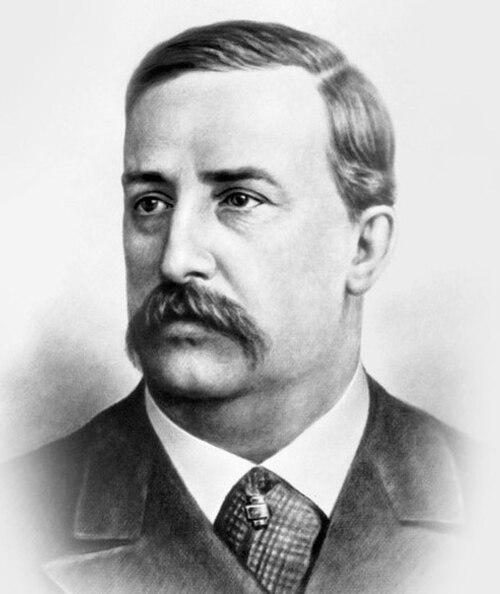
\includegraphics[width=\linewidth]{images/book3/borodin.jpg}
\end{minipage}\hspace{0.02\linewidth}%
\begin{minipage}[t]{0.18\linewidth}
\vspace{0pt}
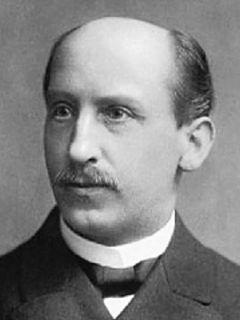
\includegraphics[width=\linewidth]{images/book3/claisen.jpg}
\end{minipage}\hfill
\begin{minipage}[t]{0.58\linewidth}
\vspace{0pt}
A reação \omterm{def:b2:enolates-aldol:aldol}{aldólica} foi descrita em 1872 por Charles-Adolphe Wurtz e, de modo independente, por
Alexander Borodin, químico de São Petersburgo hoje mais conhecido como compositor de
\textit{O Príncipe Igor}. Ludwig Claisen estendeu as condensações dos compostos carbonílicos aos
ésteres em 1887. (Retratos: Borodin, autor desconhecido, domínio público; Claisen, por
Veronica.villagrasa, CC BY-SA 4.0; Wikimedia Commons.)
\end{minipage}
\end{history}

\begin{safety}{\ghs[5mm]{GHS02}\,\ghs[5mm]{GHS05}\,\ghs[5mm]{GHS07}}
O etóxido de sódio e o di-isopropilamideto de lítio são corrosivos e reagem com a água; as soluções
de LDA são inflamáveis e manuseadas sob gás inerte. O benzaldeído e a propanona são nocivos e
inflamáveis.
% ledger: ghs:NaOEt, ghs:LDA, ghs:benzaldehyde, ghs:acetone
\end{safety}

\section{Exercícios}

\begin{exercise}[$\star$]\label{exo:b2:enolates-aldol:1}
Desenhe os \omterm{def:b2:enolates-aldol:tautomerism}{tautômeros} enólicos da butanona e da ciclo-hexanona.
\end{exercise}

\begin{exercise}[$\star$]\label{exo:b2:enolates-aldol:2}
Ordene pela acidez de sua \ce{C-H} mais ácida: propanona, pentano-2,4-diona, 3-oxobutanoato de
etila, etano.
\end{exercise}

\begin{exercise}[$\star$]\label{exo:b2:enolates-aldol:3}
Dê o \omterm{def:b2:enolates-aldol:aldol}{aldol} e o produto de condensação do etanal com o hidróxido de sódio.
\end{exercise}

\begin{exercise}[$\star$]\label{exo:b2:enolates-aldol:4}
Escreva a \omterm{def:b2:enolates-aldol:decarboxylation}{síntese malônica} do ácido hexanoico: que haloalcano é necessário?
\end{exercise}

\begin{exercise}[$\star\star$]\label{exo:b2:enolates-aldol:5}
Desenhe os \omterm{def:b2:enolates-aldol:kinetic-enolate}{enolatos cinético} e termodinâmico da 2-metilciclo-hexanona e as condições que dão
cada um.
\end{exercise}

\begin{exercise}[$\star\star$]\label{exo:b2:enolates-aldol:6}
Dê o produto da \omterm{def:b2:enolates-aldol:aldol}{condensação aldólica} cruzada do benzaldeído com a propanona (um equivalente de
cada) e explique por que o benzaldeído não se condensa consigo mesmo.
\end{exercise}

\begin{exercise}[$\star\star$]\label{exo:b2:enolates-aldol:7}
A hexano-2,5-diona em meio básico sofre uma \omterm{def:b2:enolates-aldol:aldol}{condensação aldólica} intramolecular. Que anel se forma?
Explique a escolha entre os anéis possíveis.
\end{exercise}

\begin{exercise}[$\star\star$]\label{exo:b2:enolates-aldol:8}
Escreva a \omterm{def:b2:enolates-aldol:claisen}{condensação de Claisen} do etanoato de etila e seu produto após tratamento ácido.
\end{exercise}

\begin{exercise}[$\star\star$]\label{exo:b2:enolates-aldol:9}
Quais destes dão um teste do iodofórmio positivo: propanona, pentan-3-ona, etanal, acetofenona?
\end{exercise}

\begin{exercise}[$\star\star\star$]\label{exo:b2:enolates-aldol:10}
Escreva a ciclização de Dieckmann do hexanodioato de dietila e o tamanho do anel do produto.
\end{exercise}

\begin{exercise}[$\star\star\star$]\label{exo:b2:enolates-aldol:11}
A (\textit{R})-3-metilpentan-2-ona perde sua atividade óptica em hidróxido de sódio diluído, mas a
(\textit{R})-4-metil-hexan-2-ona não. Explique.
\end{exercise}

\begin{exercise}[$\star\star\star$]\label{exo:b2:enolates-aldol:12}
Proponha uma via para a 1,5-difenilpenta-1,4-dien-3-ona, depois para uma dienona com dois grupos
arila diferentes, e diga por que a segunda é mais difícil.
\end{exercise}

\section{Problema: A dibenzalacetona}

\begin{problem}[{Problema de fim de semana --- o enolato da propanona e o papel do benzaldeído, as
duas condensações aldólicas, o produto conjugado, e a estequiometria e o rendimento de uma preparação}]
\label{pb:b2:enolates-aldol:1}
Preparação (dados do exercício): \qty{2.1}{mL} de benzaldeído e \qty{0.75}{mL} de propanona são agitados
em etanol com hidróxido de sódio aquoso; cristais amarelos de 1,5-difenilpenta-1,4-dien-3-ona
(dibenzalacetona) se separam; rendimento de 75~\%. Massas específicas (\unit{g/cm^3}): benzaldeído 1.045,
propanona 0.7845. Massas molares (\unit{g/mol}): C 12.011, H 1.008, O 15.999.
% ledger: rho:benzaldehyde, rho:acetone, aw:C, aw:H, aw:O, ghs:dibenzalacetone

\medskip
\noindent\textbf{Parte I --- Os parceiros.}
\begin{enumerate}
  \item Que parceiro tem hidrogênios $\alpha$? Quantos?
  \item Desenhe o \omterm{def:b2:enolates-aldol:enolate}{enolato} da propanona.
  \item Por que o benzaldeído não pode formar um \omterm{def:b2:enolates-aldol:enolate}{enolato}?
  \item Por que a propanona reage com o benzaldeído e não consigo mesma?
  \item Por que um aldeído é um eletrófilo melhor que uma cetona?
  \item Por que o hidróxido basta aqui como base?
\end{enumerate}

\medskip
\noindent\textbf{Parte II --- O mecanismo.}
\begin{enumerate}[resume]
  \item Escreva a adição do \omterm{def:b2:enolates-aldol:enolate}{enolato} ao benzaldeído.
  \item Escreva a desidratação do \omterm{def:b2:enolates-aldol:aldol}{aldol} formado.
  \item Por que a desidratação é fácil aqui?
  \item Por que a reação pode ocorrer uma segunda vez?
  \item Escreva a equação global.
  \item O que leva a reação até o fim nesta preparação?
\end{enumerate}

\medskip
\noindent\textbf{Parte III --- O produto.}
\begin{enumerate}[resume]
  \item Quantas ligações duplas \ce{C=C} a dibenzalacetona tem, e de que configuração (principalmente)?
  \item Por que o isômero (\textit{E},\textit{E}) é favorecido?
  \item Conte as ligações $\pi$ conjugadas.
  \item Por que o composto é amarelo enquanto seus parceiros são incolores?
  \item A dibenzalacetona é quiral?
\end{enumerate}

\medskip
\noindent\textbf{Parte IV --- Estequiometria e rendimento.}
\begin{enumerate}[resume]
  \item Calcule as massas molares do benzaldeído, da propanona e da dibenzalacetona.
  \item Calcule as quantidades dos dois reagentes.
  \item Qual reagente é o limitante?
  \item Calcule a massa teórica de produto.
  \item Por que um leve excesso de benzaldeído é preferível a um excesso de propanona?
  \item O que daria um excesso de propanona?
  \item Dê a massa de dibenzalacetona obtida com 75~\% de rendimento.
\end{enumerate}
\end{problem}
